\documentclass{article}
\usepackage{tikz}
\usepackage{pgfplots}
\usepackage{svg}
\usepackage{amsmath}
\usepackage{array}
\usepackage[skins]{tcolorbox}
\usepackage[version=4]{mhchem}
\usepackage[a4paper, total={6in, 9in}]{geometry}
\usepackage{fourier}
\usepackage{xymtex}
\usepackage{textcomp}
\usepackage{eurosym}
\usepackage{caption}
\usepackage{longtable}
\usepackage{float}
\usepackage{attachfile}
\usepackage{multirow}
\usepackage{float}
\usepackage{amsfonts} 
\usepackage[table,xcdraw]{xcolor}
\usepackage{booktabs}
\usepackage{colortbl}

\captionsetup[table]{name=\textit{Tabella}}
\pagenumbering{gobble}
%\setcounter{secnumdepth}{2}

\renewcommand*\contentsname{Indice}
\setcounter{tocdepth}{3}
\setcounter{secnumdepth}{2}
\pgfplotsset{compat=1.15}


\title{Relazione di laboratorio - Esperienza di Poisson}
\author{Federico Cesari}
\date{Marzo 2024}




\begin{document}
\begin{titlepage}
   \begin{center}
       \vspace*{1cm}
        
       \textbf{\LARGE Relazione di laboratorio - Esperienza di Poisson}
       
       \vspace{0.3cm}
       \large \textit{Rate di una sorgente radioattiva} \\
       
       \vspace{0.5cm}
       \Large Federico Cesari \\
       
       \small 1096759

			
		\vspace{1cm}
		\begin{center}
			\includegraphics[scale=1.2]{geiger.jpeg}	
		\end{center}
		
		

       \vfill
            
       
            
       \vspace{0.8cm}
     
       
            
       corso A\\
       Università degli studi di Torino, Torino\\
       3 marzo 2024\\
       
            
   \end{center}
\end{titlepage}

\tableofcontents

\newpage
\textcolor{white}{.}
\vfill


\section{Scopo dell’esperienza}

\section{Premesse teoriche}

\section{Scelta strumento di misura}

\begin{table}[]
	\centering
	\begin{tabular}{@{}clll@{}}
		\toprule
		\rowcolor[HTML]{68CBD0} 
		\textbf{$\theta$}            & \textbf{Cronometro analogico} & \textbf{Cronometro digitale} & \textbf{Fotocellula} \\ \midrule
		&                               &                              &                      \\ \cmidrule(l){2-4} 
		\multirow{-2}{*}{$10^\circ$} &                               &                              &                      \\ \midrule
		&                               &                              &                      \\ \cmidrule(l){2-4} 
		\multirow{-2}{*}{$30^\circ$} &                               &                              &                      \\ \bottomrule
	\end{tabular}
	\caption{}
	\label{tab:my-table}
\end{table}


\section{Dipendenza dall’angolo}
\subsection{Fit lineare}
\subsection{Fit parabolico}
\subsection{g}

\section{Dipendenza dalla lunghezza}
\subsection{Fit lineare}
\subsection{Confronto parametri retta}

\section{Dipendenza dalla massa}


\section{Conclusioni}














%%%%%%%%%%%%%%%%%%%%%%%%%%%%%%%%%%%%%%%%%%%%%%%%%%%%%%%%%%%%%%%%%%%%%%%%%
%%                            GRAFICI                                  %%
%%%%%%%%%%%%%%%%%%%%%%%%%%%%%%%%%%%%%%%%%%%%%%%%%%%%%%%%%%%%%%%%%%%%%%%%%



\newpage
\begin{figure}
	\centering
	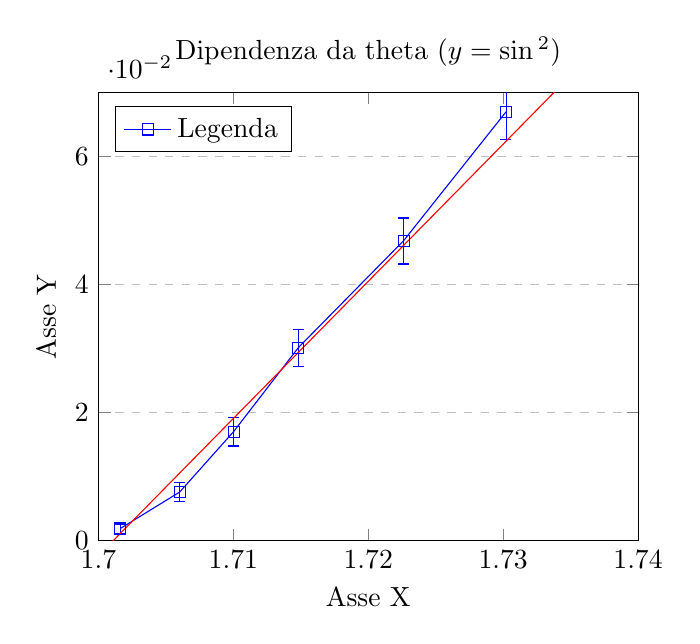
\begin{tikzpicture}
		\begin{axis}[
			title={Dipendenza da theta ($y = \sin{}^2$)},
			xlabel={Asse X},
			ylabel={Asse Y},
			xmin=1.7, xmax=1.74,
			ymin=0, ymax=0.07,
			xtick={1.7,1.71,1.72,1.73,1.74},
			ytick={0,0.02,0.04,0.06},
			legend pos=north west,
			ymajorgrids=true,
			grid style=dashed,
			]
			
			\addplot[
			color=blue,
			mark=square,
			error bars/.cd,
			y dir=both, y explicit
			]
			coordinates {
				(1.7016,0.0019027) +- (0,0.00074082)
				(1.706,0.0075961) +- (0,0.00147601)
				(1.710,0.0170371) +- (0,0.00219996)
				(1.7148,0.0301537) +- (0,0.00290717)
				(1.7226,0.0468461) +- (0,0.00359226)
				(1.7302,0.0669873) +- (0,0.00425000)
			};
			\addplot[
			domain=0:3, % Definisce l'intervallo per x
			samples=100, % Numero di punti per disegnare la retta
			color=red, % Colore della retta
			] 
			{ 2.1418758316740423*x + -3.6434786174121427}; 
			\legend{Legenda}
		\end{axis}
	\end{tikzpicture}
	\caption{Didascalia del grafico.}
\end{figure}

\begin{figure}
	\centering
	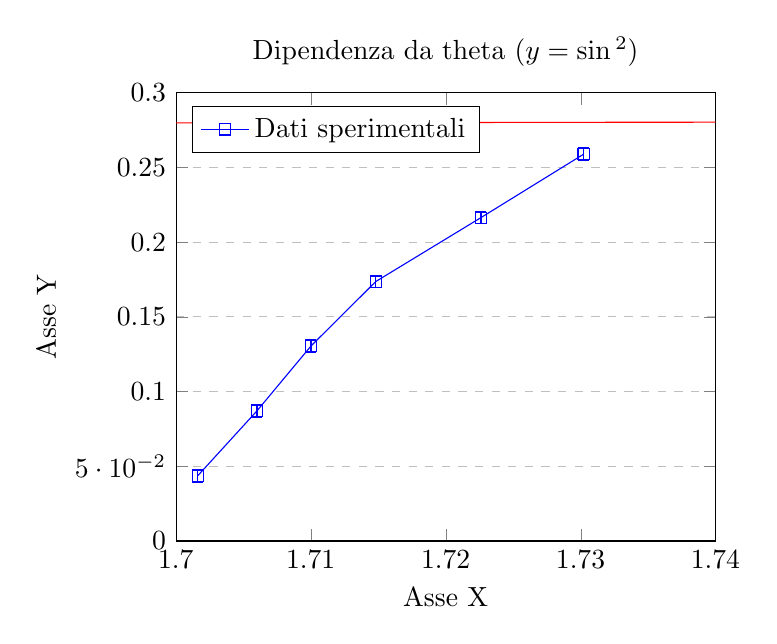
\begin{tikzpicture}
		\begin{axis}[
			title={Dipendenza da theta ($y = \sin{}^2$)},
			xlabel={Asse X},
			ylabel={Asse Y},
			xmin=1.7, xmax=1.74,
			ymin=0, ymax=0.3,
			xtick={1.7,1.71,1.72,1.73,1.74},
			ytick={0,0.05,0.1,0.15,0.2,0.25,0.3},
			legend pos=north west,
			ymajorgrids=true,
			grid style=dashed,
			]
			
			\addplot[
			color=blue,
			mark=square,
			error bars/.cd,
			y dir=both, y explicit
			]
			coordinates {
				(1.7016,0.0436194) +- (0,0.004345)
				(1.706,0.0871557) +- (0,0.004333)
				(1.710,0.1305262) +- (0,0.0043128)
				(1.7148,0.1736482) +- (0,0.0042839)
				(1.7226,0.2164396) +- (0,0.0042469)
				(1.7302,0.2588190) +- (0,0.0042018)
			};
			\addplot[
			domain=0:3, % Definisce l'intervallo per x
			samples=100, % Numero di punti per disegnare la parabola
			color=red, % Colore della parabola
			] 
			{-0.027555*x^2 + 0.106957*x + 0.17762}; 
			\legend{Dati sperimentali}
			\legend{Dati sperimentali}
		\end{axis}
	\end{tikzpicture}
	\caption{Didascalia del grafico illustrante l'andamento dei dati con errori.}
\end{figure}

\begin{figure}
	\centering
	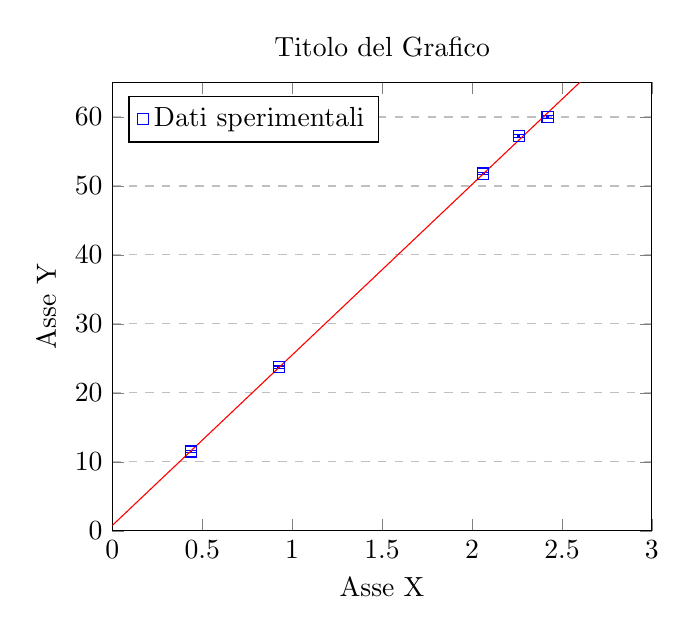
\begin{tikzpicture}
		\begin{axis}[
			title={Titolo del Grafico},
			xlabel={Asse X},
			ylabel={Asse Y},
			xmin=0, xmax=3,
			ymin=0, ymax=65,
			xtick={0,0.5,1,1.5,2,2.5,3},
			ytick={0,10,20,30,40,50,60},
			legend pos=north west,
			ymajorgrids=true,
			grid style=dashed,
			]
			
			\addplot[
			color=blue,
			mark=square,
			only marks,
			error bars/.cd,
			y dir=both, y explicit,
			error bar style={line width=1pt}
			]
			coordinates {
				(2.25961024,57.20) +- (0,0.2)
				(0.925444,23.70) +- (0,0.2)
				(0.43797924,11.50) +- (0,0.2)
				(2.41989136,60.00) +- (0,0.2)
				(2.062096,51.80) +- (0,0.2)
			};
			\addplot[
			domain=0:3, % Definisce l'intervallo per x
			samples=100, % Numero di punti per disegnare la retta
			color=red, % Colore della retta
			] 
			{24.71884439277015*x + 0.7706502111761893}; 
			\legend{Dati sperimentali}
		\end{axis}
	\end{tikzpicture}
	\caption{Didascalia del grafico illustrante l'andamento dei dati con errori.}
\end{figure}




\end{document}
